% !TEX root=/home/tavant/these/manuscript/src/manuscript.tex

\section{Characteristics of the azimuthal instability}

\inlinenote{Here, 
Discuss on the saturation by ion trapping via the same equation as \cref{subsec-temp}.  }

The case defined by Boeuf is more efficient to  study the instability.
Indeed, at the ionization is not self-consistent, it removes the breathing mode.
Hence, we will focus on the results obtained with Boeuf model this section.
We recall that thee cases have been simulated\string: the nominal case without radial losses and two other cases with the radial losses modeled with $L_R=2\,\centi\meter$ and $L_R=4\,\centi\meter$.

\subsection{Overview of the azimuthal instability} \label{subsec-label}
\Cref{fig-snapshots} shows the azimuthal electric field at the end of the simulations for the three cases.
We can see the azimuthal instability in all of the simulation domain.
We note that the radial losses do not modify significantly the instability.
From the characteristics of the instability seen in \cref{fig-snapshots}, two zones can be discerned\string:
\begin{itemize}
  \item The upstream region, $z < 8 \,\milli\meter$, the instability present a short wavelength, and is oblique.
  \item The downstream region, $z > 1\,\centi\meter$, the wavelength of the instability is larger and is almost perfectly azimuthal.
\end{itemize}
The radial losses seems to reduce the wavelength of the instability in both the upstream and the downstream regions.


\begin{figure}[hbtp]
  \centering
  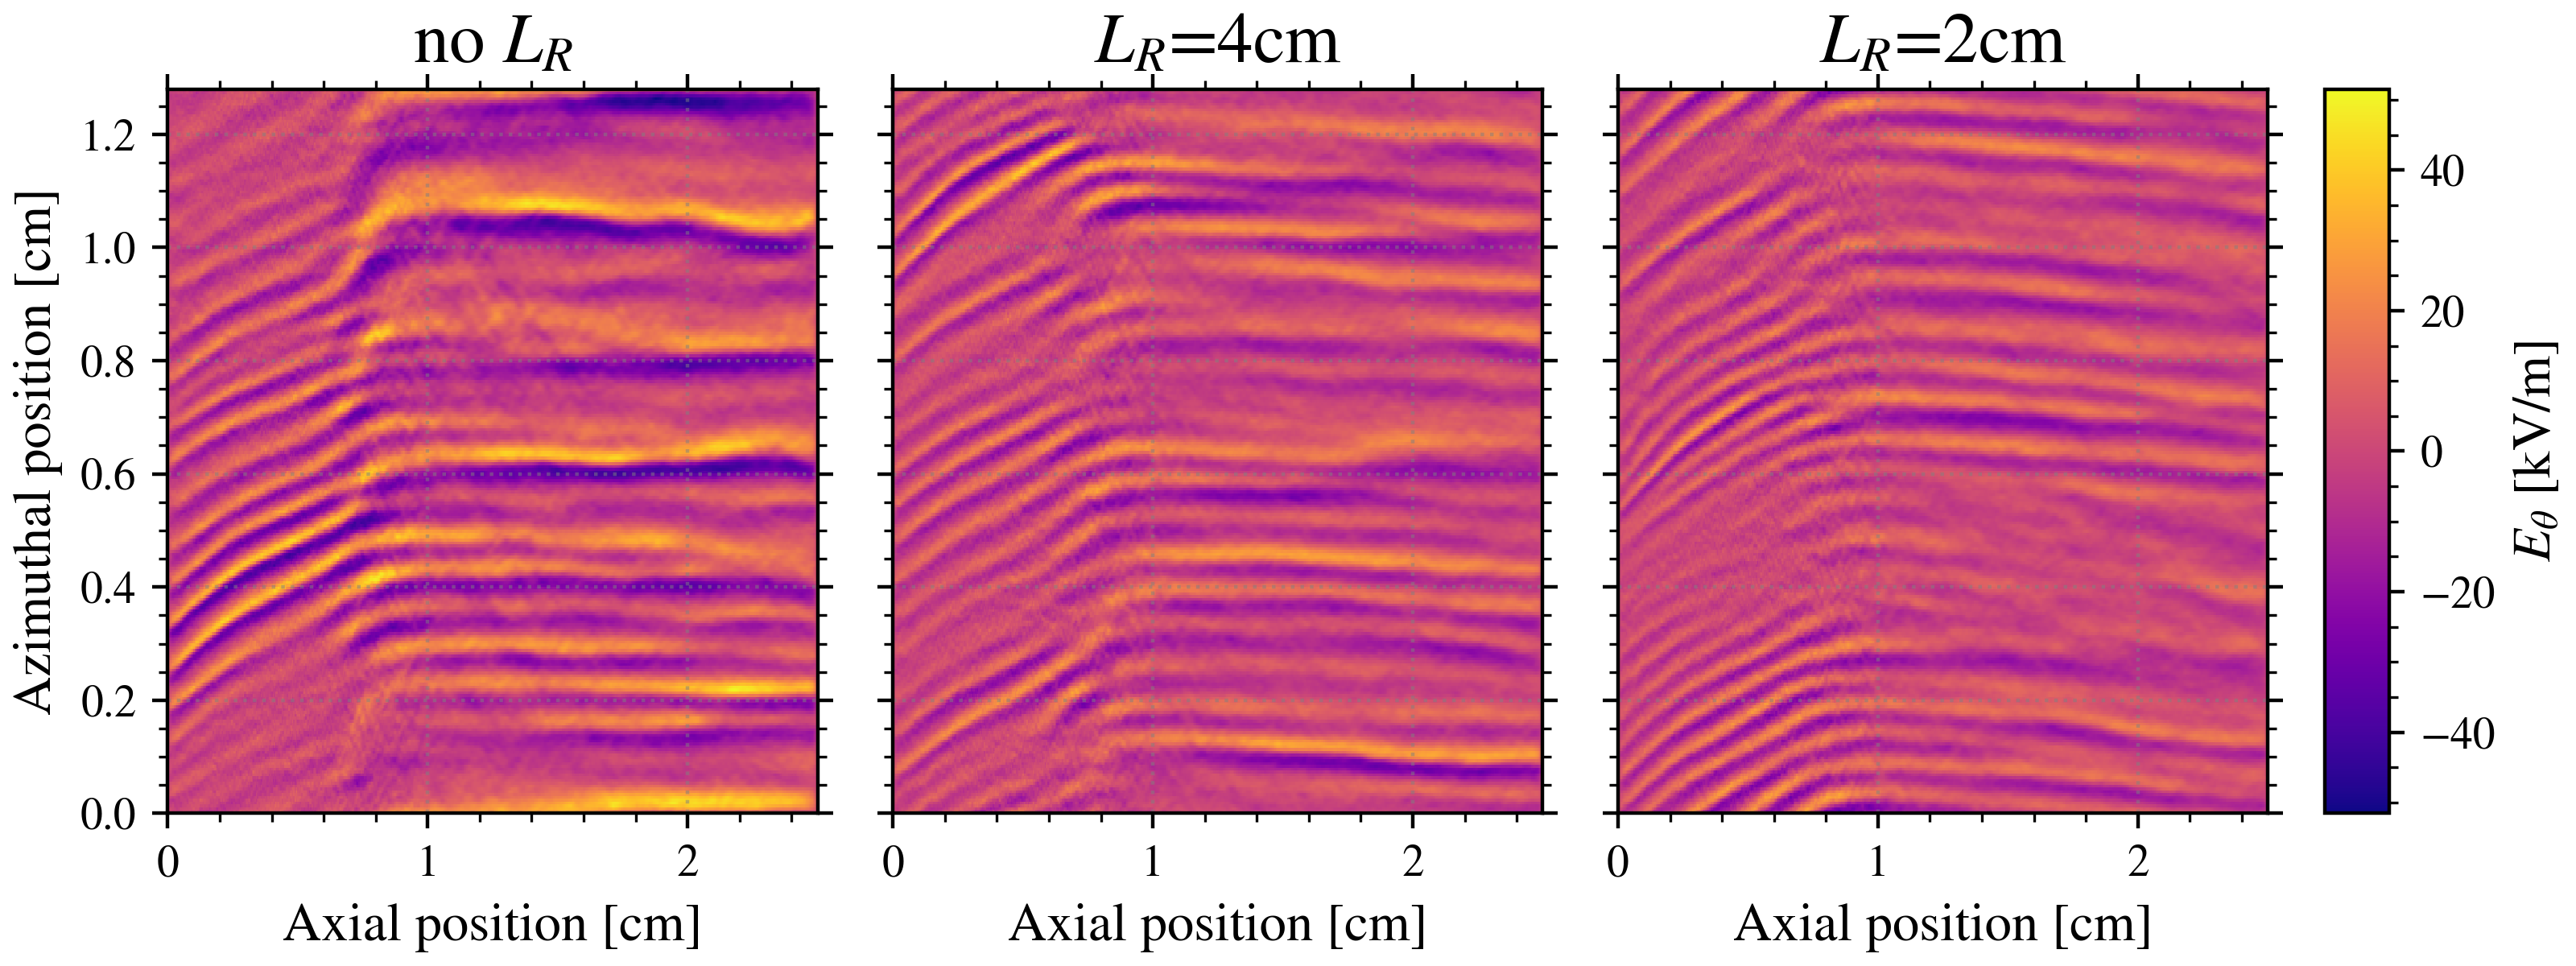
\includegraphics[width=\textwidth]{Boeuf_Ex_snapshot}
  \caption{Azimuthal electric field obtained at the end of the simulation for the three cases using the model of Boeuf.}
  \label{fig-snapshots}
\end{figure}

We have seen in \cref{ch-5} that the instability wavelength is of the order of the Debye length $\lde$ and its frequency of the order of the ion plasma frequency $\opi$.
\Cref{fig-wpi_Lde} shows the axial evolution of the ion plasma frequency and the Debye length for the three cases.
Because of the large anisotropy of the electron temperature, the Debye length is calculated using the azimuthal temperature $\Te_{\theta}$.
We can see that $\opi$ is not significantly affected, in the upstream region, but decreases with the increase of the losses in the downstream region.

\begin{figure}[hbtp]
  \centering
  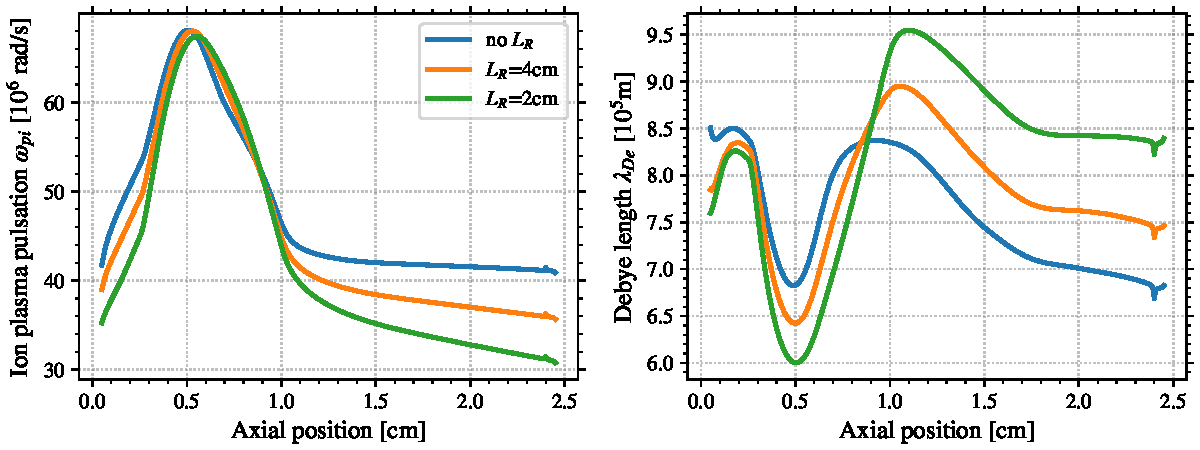
\includegraphics[width=\textwidth]{Boeuf_opi_Lde}
  \caption{Axial evolution of (right) the ion plasma frequency and (left) the Debye length for the three cases using the model of Boeuf.}
  \label{fig-wpi_Lde}
\end{figure}

Concerning the Debye length, we can see in \cref{fig-wpi_Lde} that the radial losses change $\lde$ in both region, but not is the same order.
In the upstream region, the radial losses decrease $\lde$, while they increase $\lde$ in the downstream region.
This means that the evolution of the wavelength observed in \cref{fig-snapshots} is not due to the differences in the Debye length.

\subsection{Spectral analyses of the waves} \label{subsec-fft}

We proceed to a quantitative analyze of the instability, to better understand the modifications of the instability.
The spectral analyses are perfomed at $z_u=0.25\,\centi\meter$ for the upstream region, and $z_d=1.5\,\centi\meter$ for the downstream region.
\Cref{fig-cut2D} shows the temporal evolution of the azimuthal electric field $E_{\theta}$ when no radial losses are modeled for $z_u$ and $z_d$.

\begin{figure}[hbtp]
  \centering
  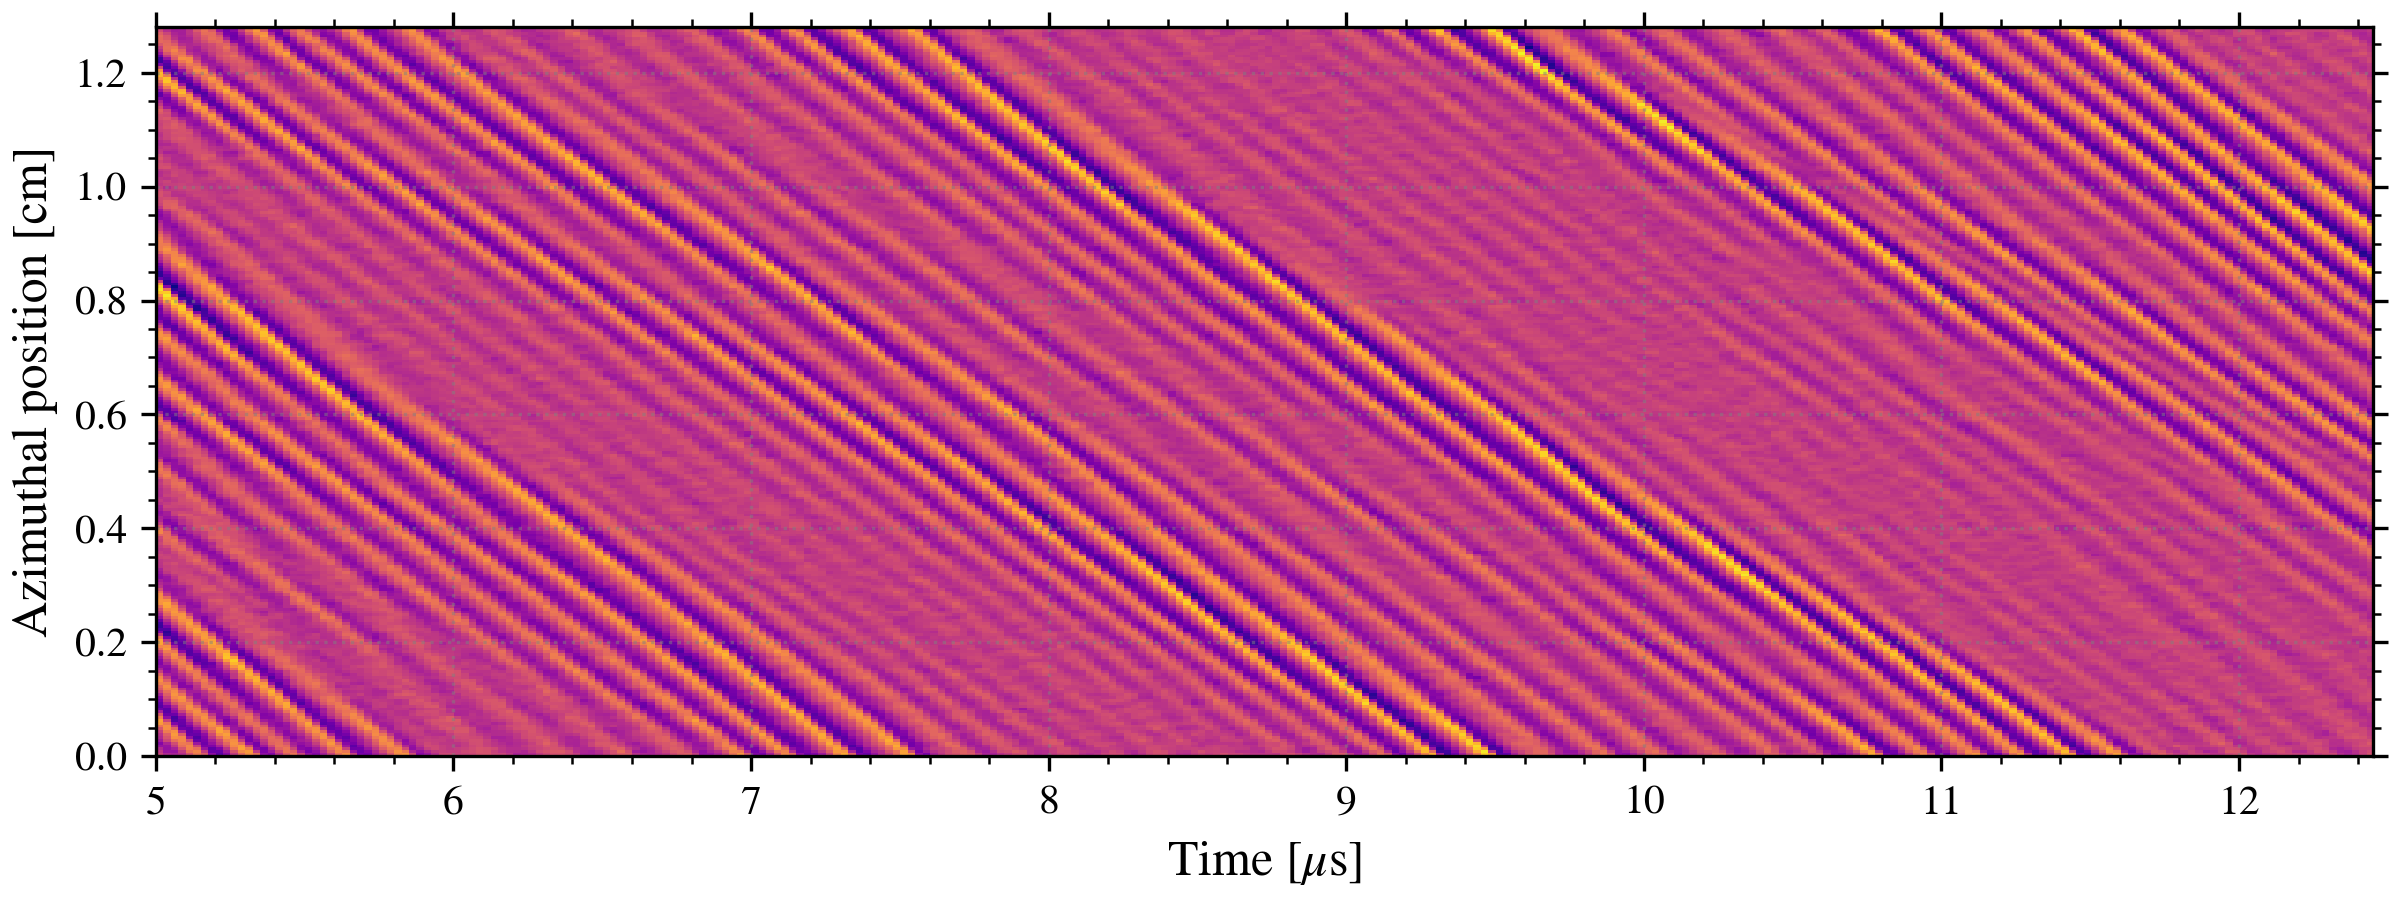
\includegraphics[width=\textwidth]{Boeuf_noLr_y50_t200}
  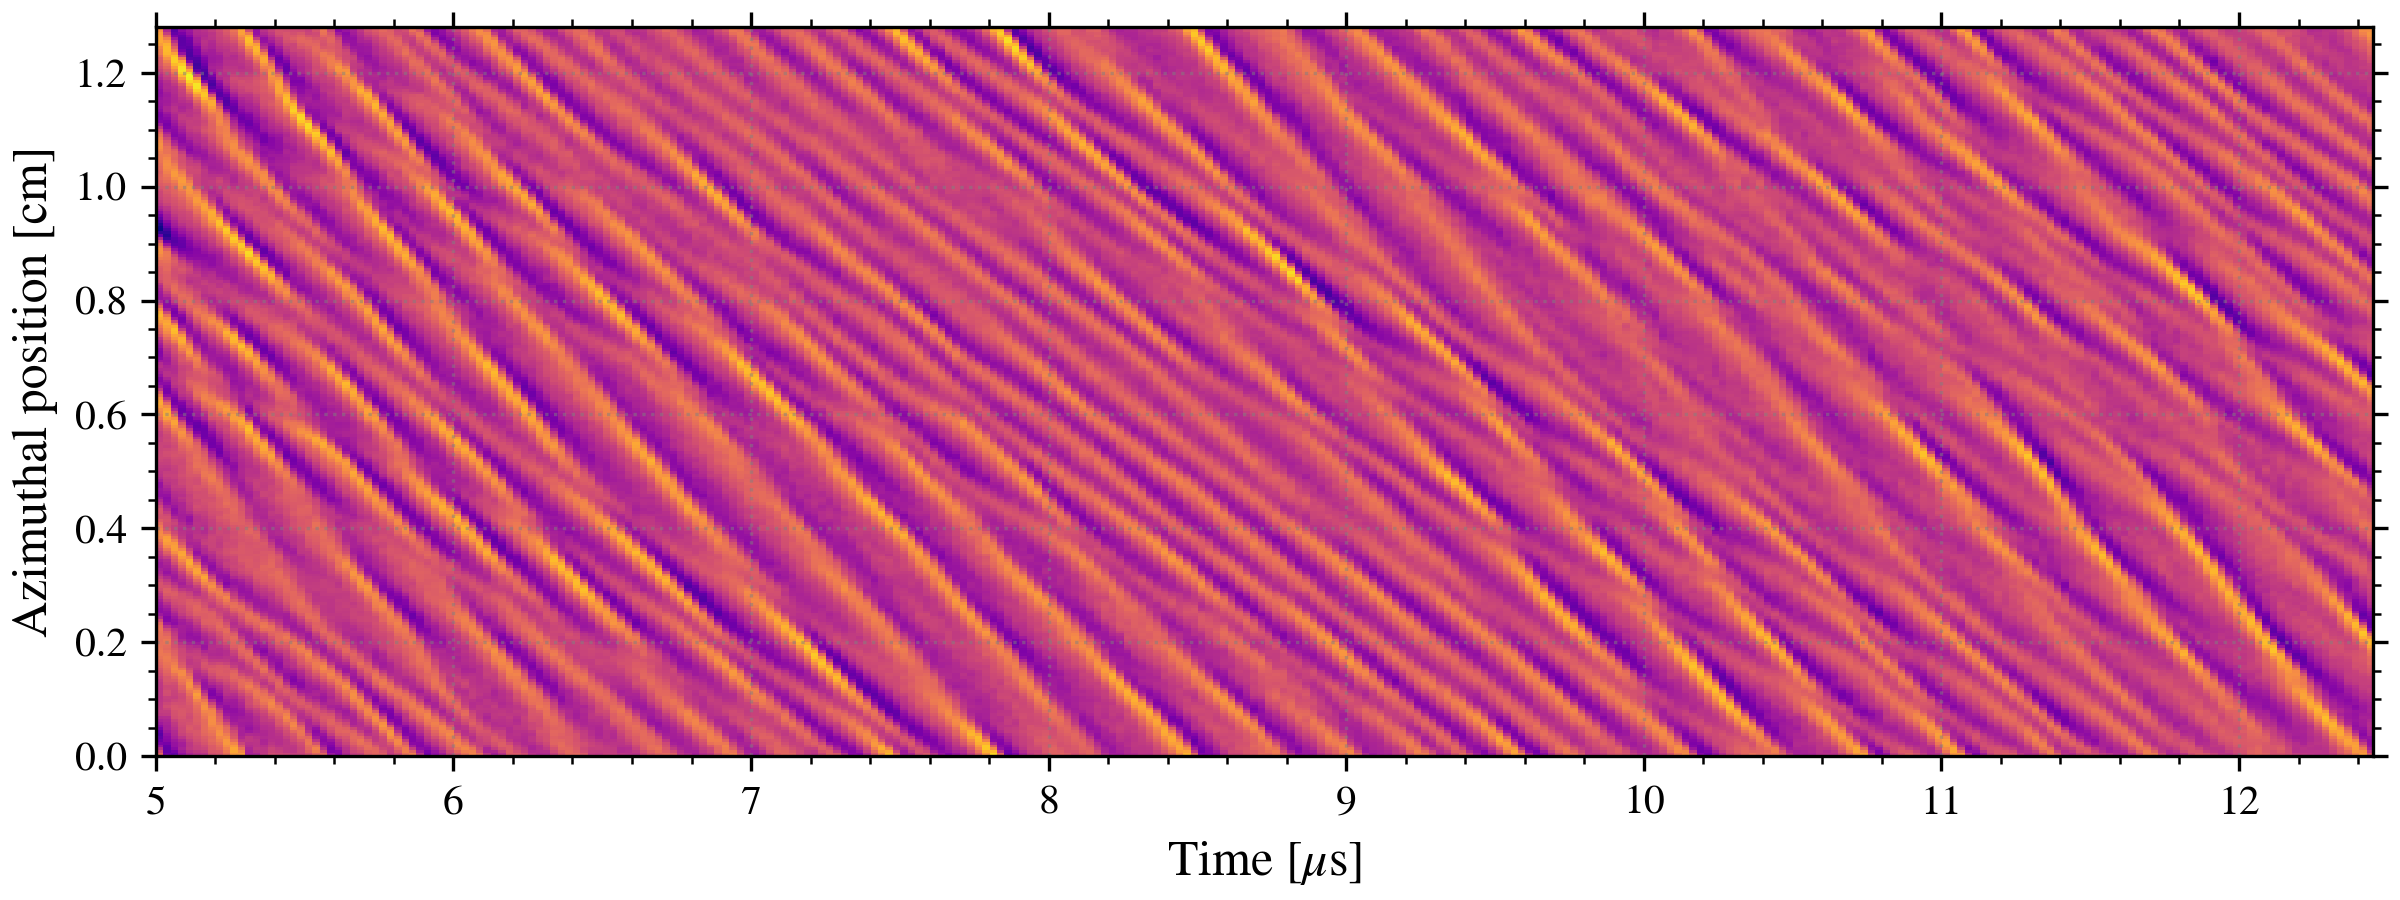
\includegraphics[width=\textwidth]{Boeuf_noLr_y300_t200}
  \caption{Spatio-temporal evolution of the azimuthal electric field at (top) $z=z_u$ and (bottom) $z=z_d$ when no instability are present. The beginning of the simulation ($t<5\,\micro\second$) are removed, because the wave is not yet saturated. }
  \label{fig-cut2D}
\end{figure}


For the upstream region, the wave is clear. 
We can see a modulation of the amplitude of the wave, and it seems that the group velocity of the wave is smaller than the phase velocity.
The downstream region is more complex, as there is a combination of two waves.
We perform a \ac{2D} \ac{FFT} on the spatio-temporal azimuthal electric field to obtain the relation dispersion of the wave observed.
\Cref{fig-fft2D_noLr_zu} shows the \ac{2D} \ac{FFT} in the upstream region.
We also display the \ac{1D} \ac{FFT} obtained by summing the \ac{2D} \ac{FFT} in one direction.
We can see that the waves follow one well-defined curve, wich is close to the \ac{IAW} of \cref{eq-MIAW} using the local Debye length and ion plasma pulsation.
The maximum of the wave is located at $k_{\theta} = 8.5\,\radian\per\milli\meter$ and $\omega = 35\, \radian\per\mega\hertz$.

\begin{figure}[hbtp]
  \centering
  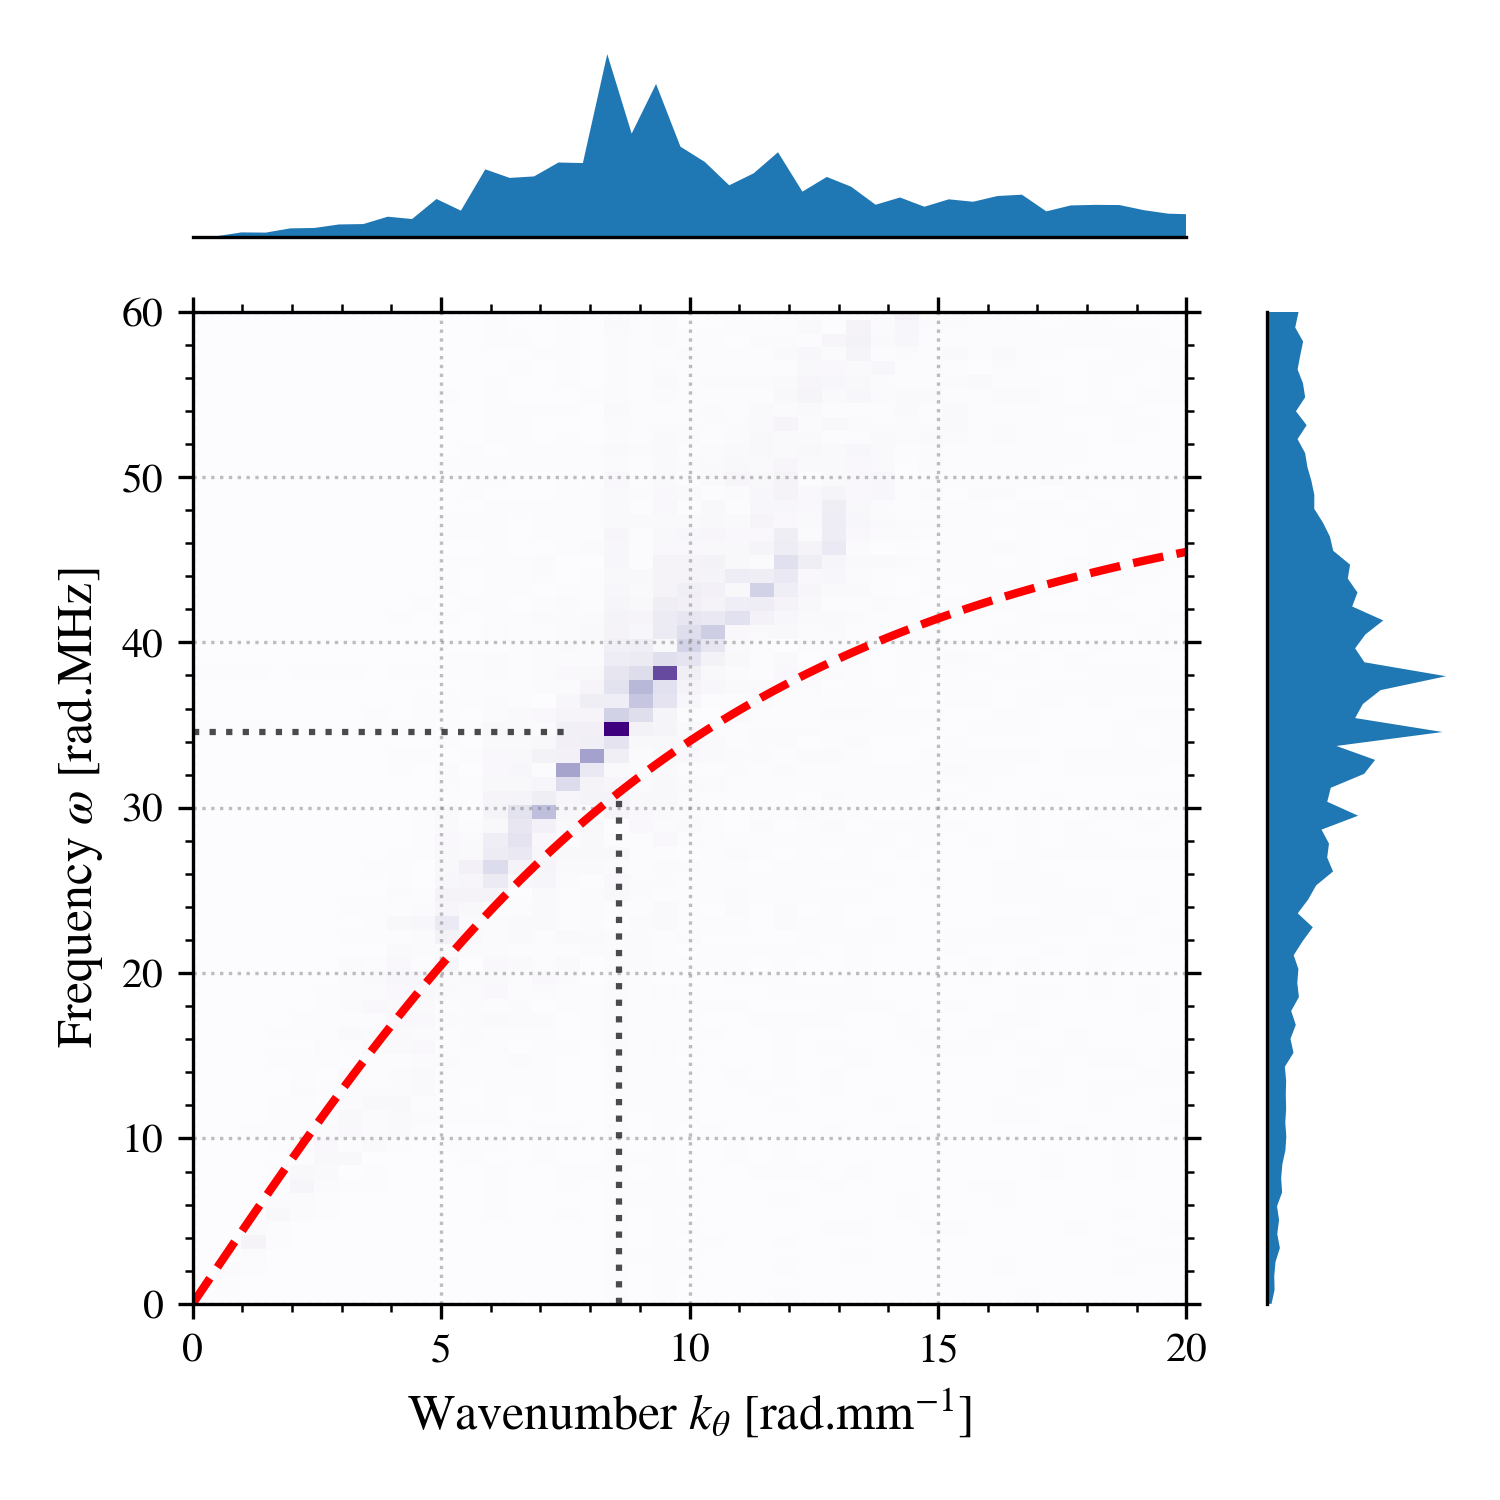
\includegraphics[width=5in]{Boeuf_noLr_FFT2D_y50_full}
  \caption{\ac{2D} and \ac{1D} \ac{FFT} of the azimuthal electric field in the upstream region $z=z_u$ without radial losses. The black dotted lines highlight the position of the maximum of the \ac{2D} \ac{FFT}. The red dash line corresponds the the \ac{IAW} dispersion relation of \cref{eq-MIAW}.}
  \label{fig-fft2D_noLr_zu}
\end{figure}

The \ac{2D} \ac{FFT} in the downstream region is presented in \cref{fig-fft2D_noLr_zd}.
In contrast to the upstream region, we can see that the waves do not follow one well-defined curve.
The maximum of the wave is located at $k_{\theta} = 3\,\radian\per\milli\meter$ and $\omega = 20\, \radian\per\mega\hertz$.
The wave characteristics of the upstream region can still be seen, but a larger and slower wave is overlaid to it.
However, this new wave seems to follow the same dispersion relation as in the upstream, but not the one using the local plasma parameters, which underestimates the waves parameters.


\begin{figure}[hbtp]
  \centering
  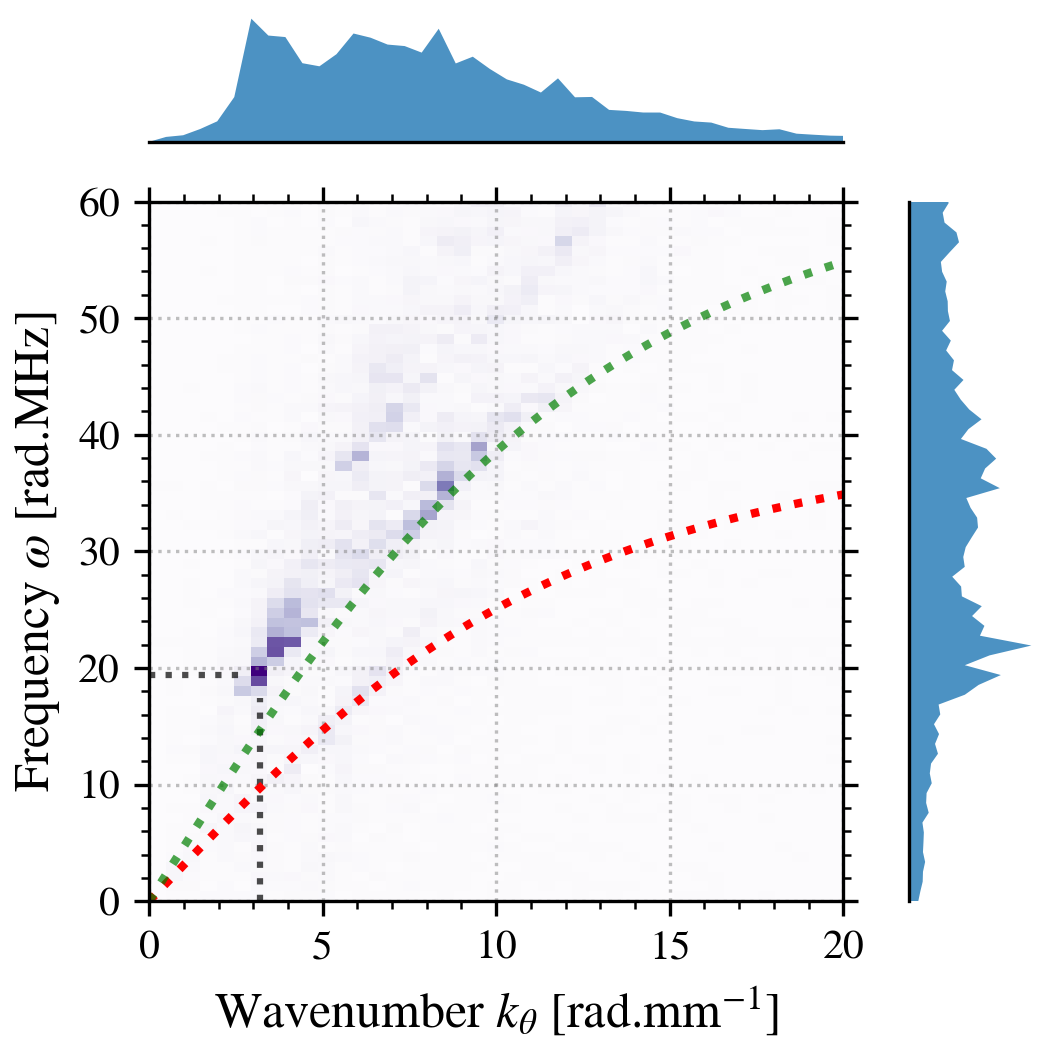
\includegraphics[width=5in]{Boeuf_noLr_FFT2D_y300_full}
  \caption{\ac{2D} and \ac{1D} \ac{FFT} of the azimuthal electric field in the downstream region $z=z_d$ without radial losses.  The black dotted lines highlight the position of the maximum of the \ac{2D} \ac{FFT}, and the red dash line corresponds the the \ac{IAW} dispersion relation of \cref{eq-MIAW}.}
  \label{fig-fft2D_noLr_zd}
\end{figure}

\subsection{Impact of the radial losses on the \ac{FFT}} \label{subsec-fft_losses}

\Cref{fig-fft2D_Lr4_zd,fig-fft2D_Lr2_zd} show the \ac{2D} \ac{FFT} obtained with the radial losses in the downstream region.
In the upstream region, the results are similar to the case without radial losses.
We can see that for $L_R=4\,\centi\meter$


\begin{figure}[hbtp]
  \centering
  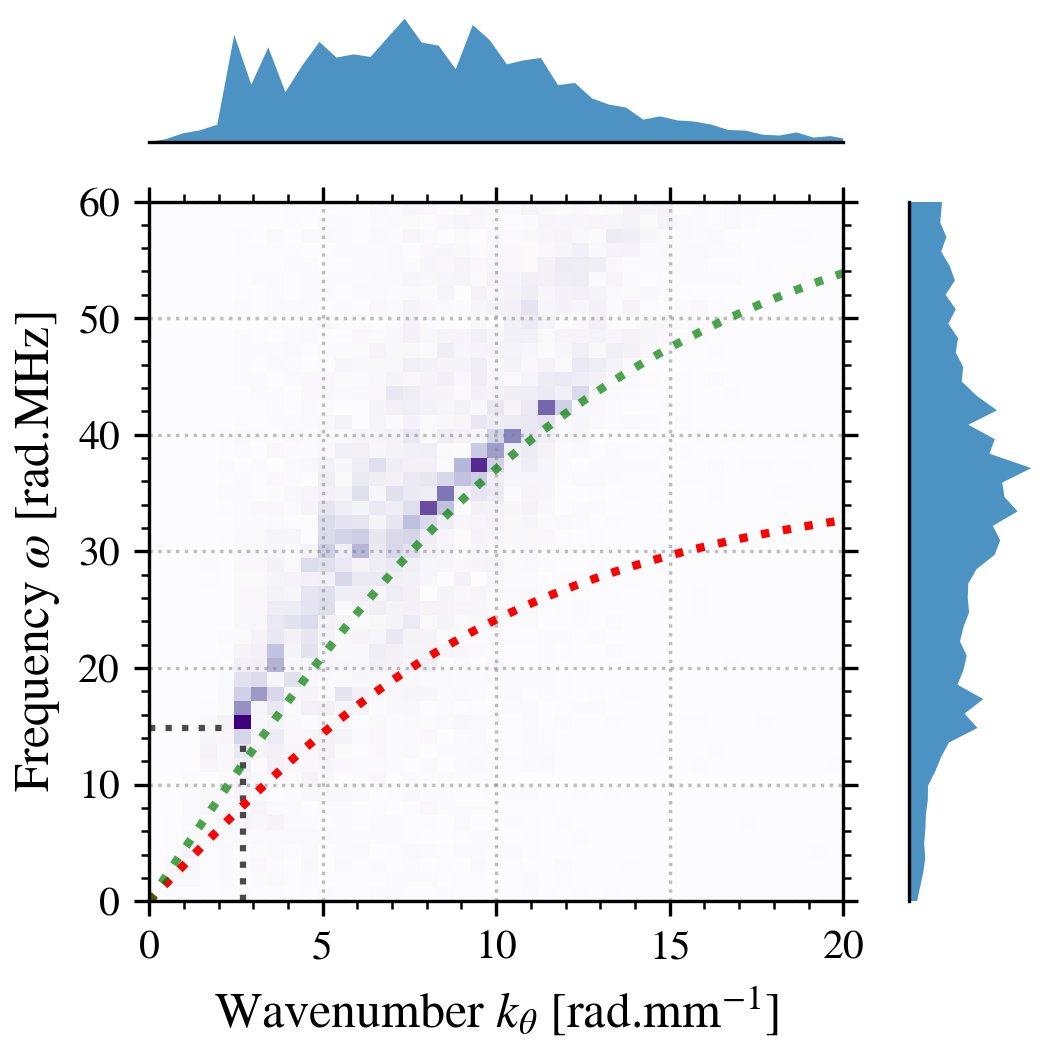
\includegraphics[width=5in]{Boeuf_Lr4_FFT2D_y300_full}
  \caption{\ac{2D} and \ac{1D} \ac{FFT} of the azimuthal electric field in the downstream region $z=z_d$ with $L_R=4\,\centi\meter$.  The black dotted lines highlight the position of the maximum of the \ac{2D} \ac{FFT}, and the red dash line corresponds the the \ac{IAW} dispersion relation of \cref{eq-MIAW}.}
  \label{fig-fft2D_Lr4_zd}
\end{figure}


\begin{figure}[hbtp]
  \centering
  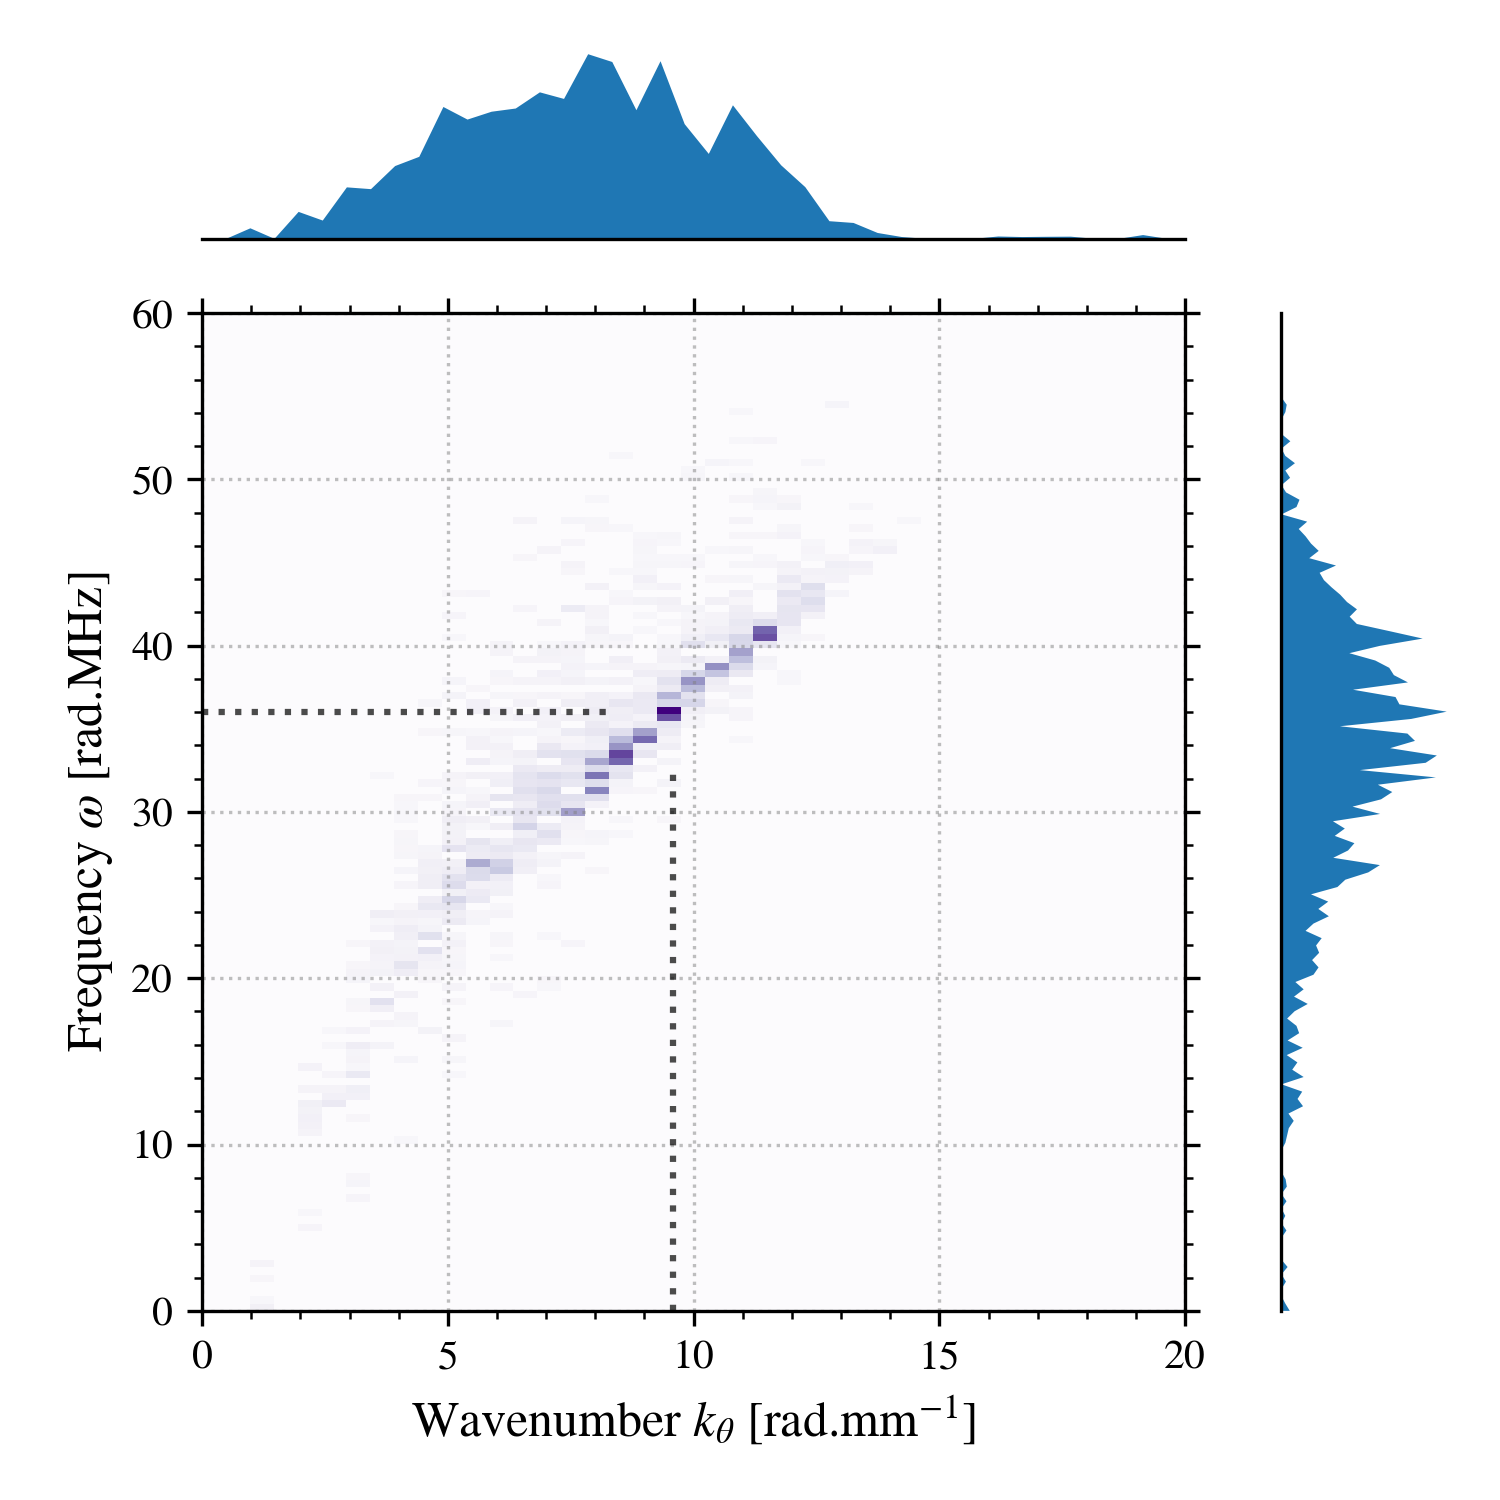
\includegraphics[width=5in]{Boeuf_Lr2_FFT2D_y300_full}
  \caption{\ac{2D} and \ac{1D} \ac{FFT} of the azimuthal electric field in the downstream region $z=z_d$ with $L_R=2\,\centi\meter$.  The black dotted lines highlight the position of the maximum of the \ac{2D} \ac{FFT}.}
  \label{fig-fft2D_Lr2_zd}
\end{figure}

\subsection{Axial evolution of the wave characteristics} \label{subsec-axial_profile}

the \ac{2D} \ac{FFT} presented in \cref{subsec-fft,subsec-fftlosses} where only given for $z=z_u$ and $z=z_d$.
In this section, we investigate the axial evolution on the wave characteristics.
To do so, we present in \Cref{fig-axial_fft1D} the axial evolution of the \ac{1D} \ac{FFT} for the three cases.
 
\begin{figure}[hbtp]
  \centering
  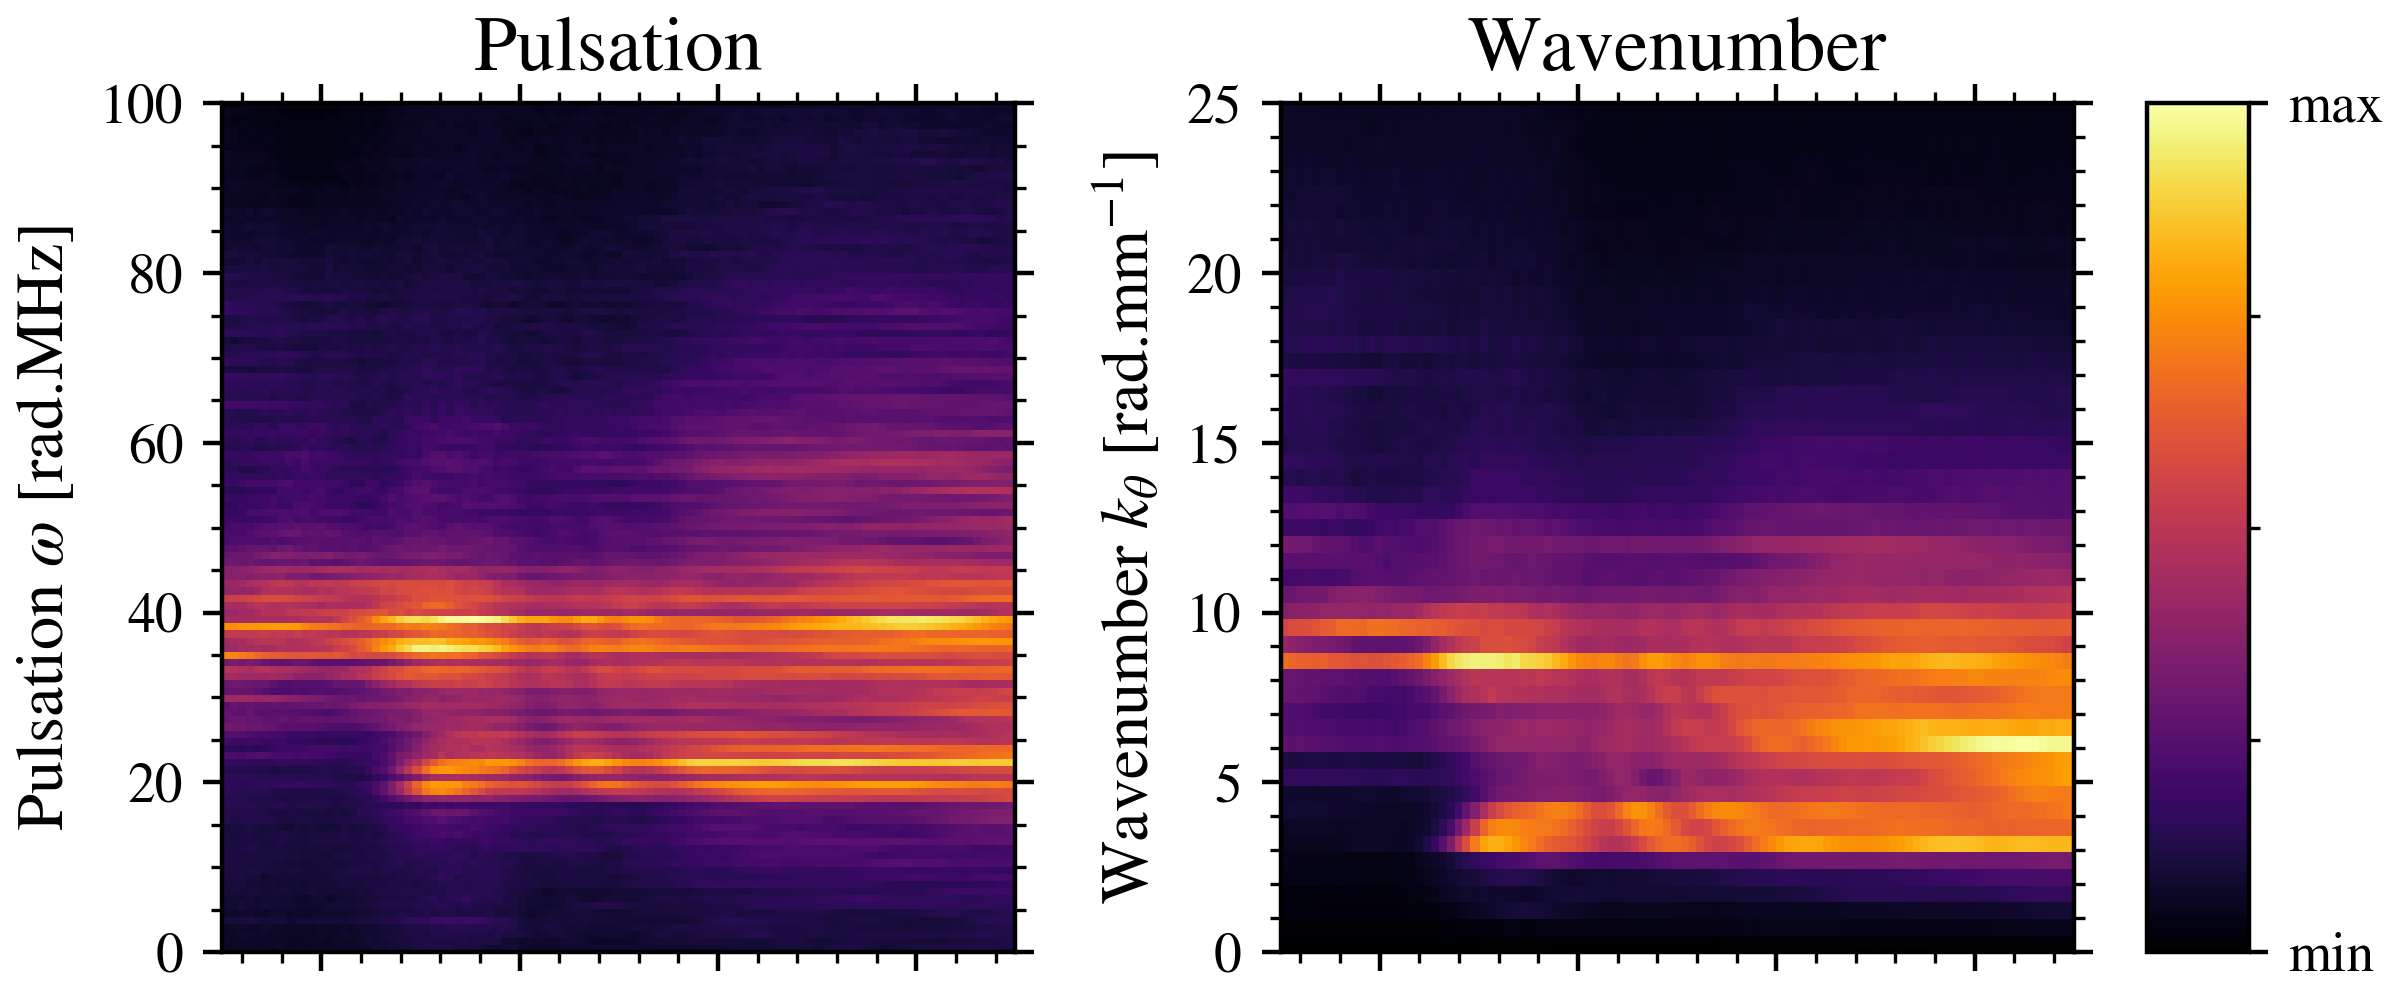
\includegraphics[width=\textwidth]{Boeuf_axila_evolution_fft1D_noLr}
  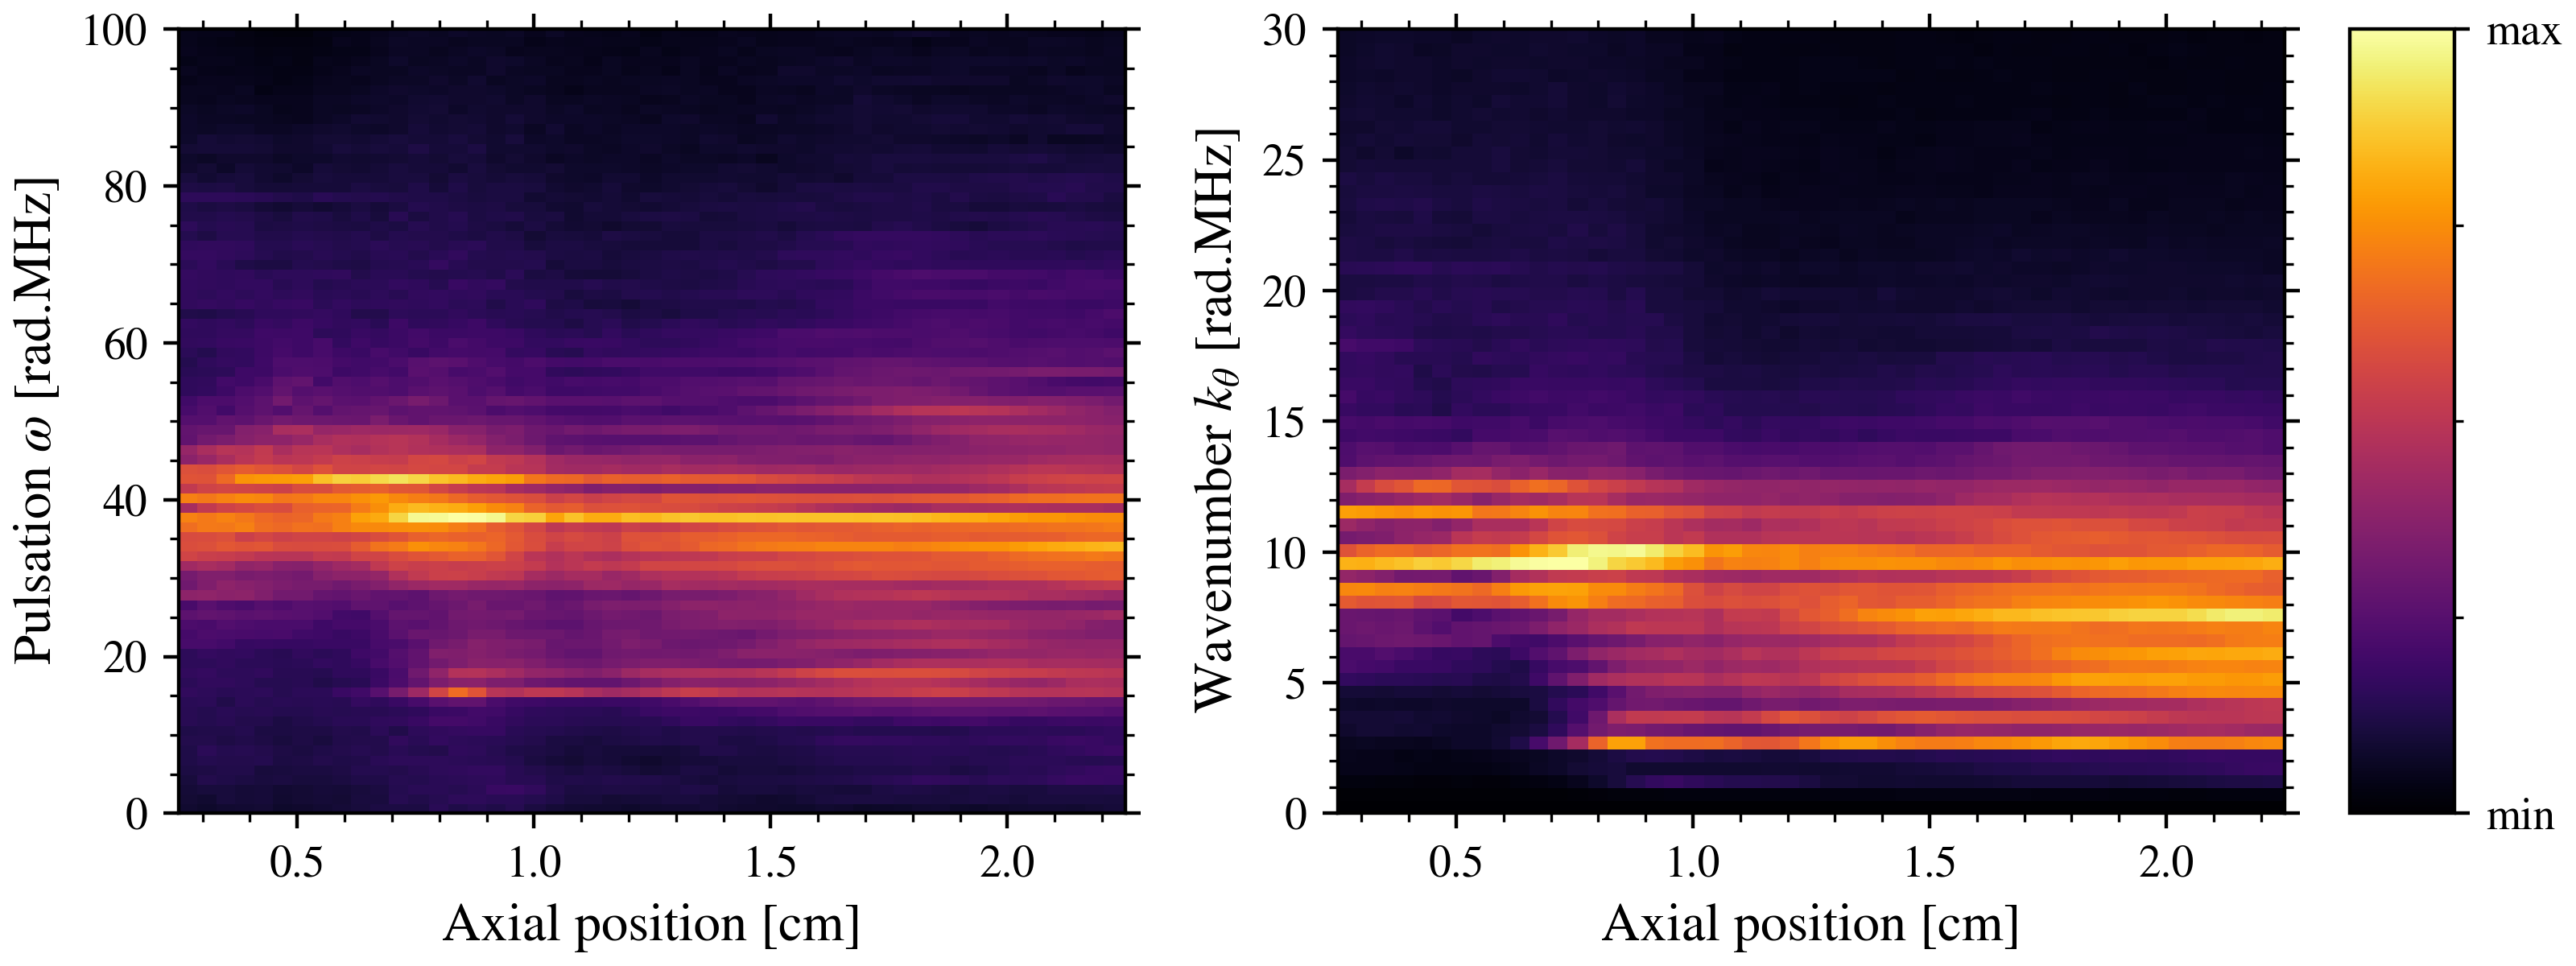
\includegraphics[width=\textwidth]{Boeuf_axila_evolution_fft1D_Lr4}
  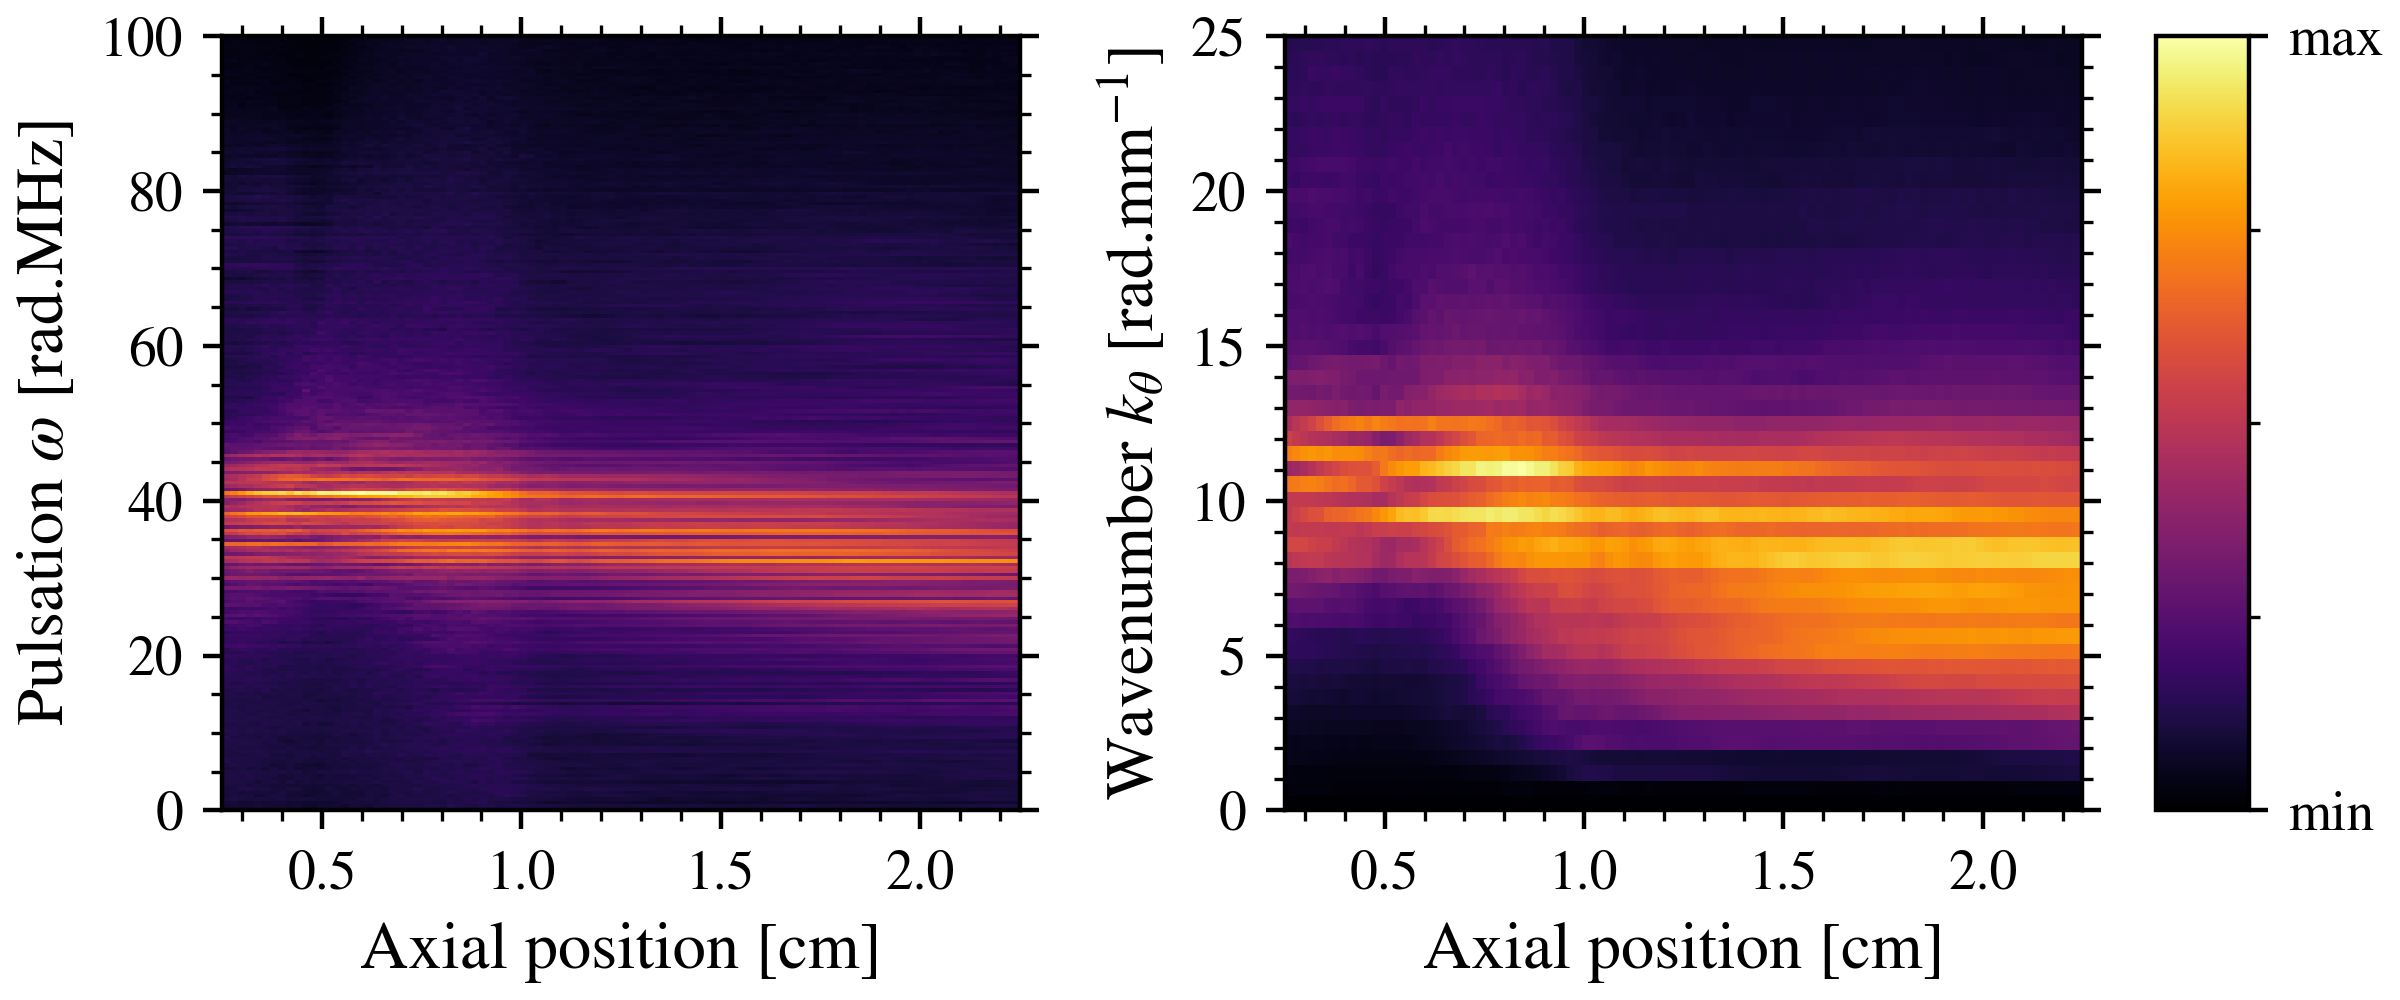
\includegraphics[width=\textwidth]{Boeuf_axila_evolution_fft1D_Lr2}
  \caption{Axial evolution of the \ac{1D} \ac{FT} on (left) the frequency and (right) the wavenumber for (top) no radial losses, (middle) $L_r=4\,\centi\meter$, and (bottom) $L_r=\,\centi\meter$ using the model of Boeuf. }
  \label{fig-axial_fft1D}
\end{figure}

We can see in \cref{fig-axial_fft1D} that the low frequency oscillation appears approximately at $z=0.75\,\centi\meter$, which corresponds to the maximum of the magnetic field.
We see that it does not replace the short-wavelength wave of the upstream region, but instead it is added to it.
This second low-frequency oscillation is clearly visible when no radial losses are present, but its amplitude is reduced for $L_R=4\,\centi\meter$.
Moreover, it is almost non-existent for $L_R=2\,\centi\meter$ in the frequency spectra, but seems to be present in the wavenumber spectra.

We have see previously that the \ac{1D} spectral aggregates the waves information, thus the larger wave cannot be directly observed by this way.
\Cref{fig-axial_maxwave_normalized} shows the axial evolution of the wave characteristics (pulsation and wavenumber) for the wave of maximum amplitude in the \ac{2D} \ac{FFT}, such as the one located by the dotted lines in \cref{fig-fft2D_noLr_zd}.
The pulsation $\omega$ is normalized by the local ion plasma pulsation $\opi$ given in \cref{fig-wpi_Lde}.
The azimuthal wavenumber $k_{\theta}$ is normalized by the local Debye length.
 
\begin{figure}[hbtp]
  \centering
  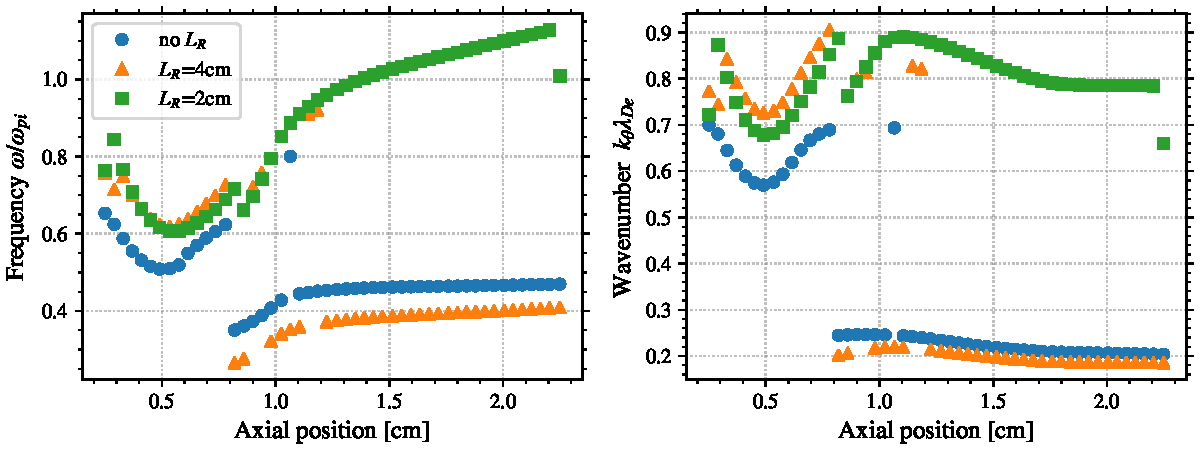
\includegraphics[width=\textwidth]{Boeuf_caracteristics_all_normalized}
  \caption{Axial evolution of (left) the frequency and (right) the wavenumber of the wave of maximum amplitude in the \ac{2D} \ac{FFT} for the three cases using the model of Boeuf. The pulsation and the wavenumber are normalized by the local ion plasma pulsation, respectively the Debye length.}
  \label{fig-axial_maxwave_normalized}
\end{figure}

We can see in \cref{fig-axial_maxwave_normalized} that the in the upstream region, the cases with radial losses ($L_R=2 and 4\,\centi\meter$) present similar waves characteristics, with higher frequency and wavenumber that the case without radial losses.
However, in the upstream region the wave of maximum amplitude is the low frequency wave for both cases without losses and with $L_r=4\,\centi\meter$.
On the other hand, the case $L_R=2\,\centi\meter$ shows a small discontinuity, but the wave characteristics are very close.


\subsection{Ion-trapping saturation } \label{subsec-boeuf_iontrapping}

The model of Boeuf allows the simulation to reach a steady-state.
We use the criteria developed in \cref{subsec-temp} and given by \cref{eq-criteriaIT} to determine whether or not the wave saturates because of ion-wave trapping.

\begin{figure}[hbtp]
  \centering
  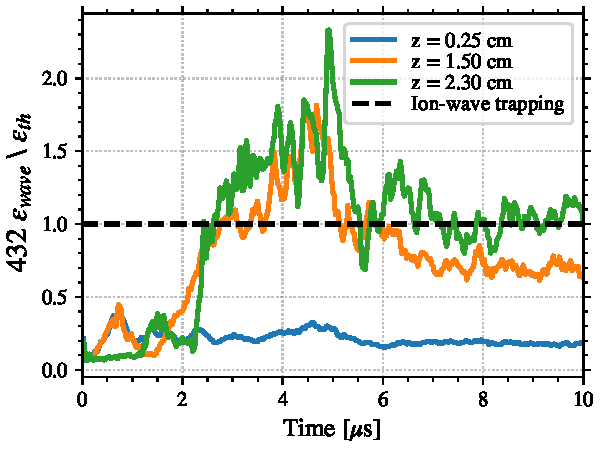
\includegraphics[width=\defaultwidth]{Boeuf_iontrapping_noLr}
  \caption{Temporal evolution of the ion-wave trapping criteria for the model of Boeuf without radial losses at three positions\string: $z=0.25\,\centi\meter$, un the upstream region; $z=1.5\,\centi\meter$, and $z=2.3\,\centi\meter$, in the downstream region.}
  \label{fig-ion-trap_temp_noLr}
\end{figure}

We can see in \cref{fig-ion-trap_temp_noLr} the temporal evolution of the ion-wave trapping criteria for the model of Boeuf without radial losses at three positions, one in the upstream region and two in the downstream region.
We can see that in the upstream region, the criterion is never reached.
On the other hand, the criteria is quickly reached in the downstream region, especially for $z=2.3\,\centi\meter$.
For $z=1.5\,\centi\meter$, the criteria is reached during approximately two microsecond between $t=3.5$ and $t=5\,\micro\second$, but then return below the threshold value.

\Cref{fig-ion-trap_temp_Lr} shows the same information than \cref{fig-ion-trap_temp_noLr} but with the radial losses modeled.
We can see that at the end of the simulations ($t=10\,\micro\second$) the criterion is no more fulfilled.
It means that the wave amplitude is smaller than the one expected with ion trapping.
\begin{figure}[hbtp]
  \centering
  \begin{tabular}{cc}
    \subfigure{Boeuf_iontrapping_Lr4}{a}{20,65} & 
    \subfigure{Boeuf_iontrapping_Lr2}{b}{20,65} \\
  \end{tabular}
  \caption{Temporal evolution of the ion-wave trapping criteria for the model of Boeuf with ({\bf a}) $L_R=4\,\centi\meter$, and ({\bf b}) $L_R=2\,\centi\meter$  at three positions\string: $z=0.25\,\centi\meter$, un the upstream region; $z=1.5\,\centi\meter$, and $z=2.3\,\centi\meter$, in the downstream region.}
  \label{fig-ion-trap_temp_Lr}
\end{figure}

\Cref{fig-ionwavetrapping_axial} shows the axial profile of the ion-wave trapping average in time between $t=6\,\micro\second$ and $t=10\,\micro\second$ for the three cases.
It confirms the observations of \cref{fig-ion-trap_temp_noLr,fig-ion-trap_temp_Lr} that the case without the radial losses reaches the criteria, while the two other case do not.
At the moment, we're not sure what the reason of this evolution is.
The radial losses reduces the electron temperature and density, hence the thermal energy.
But apparently, the amplitude of the instability diminishes more significantly.

\begin{figure}[hbtp]
  \centering
  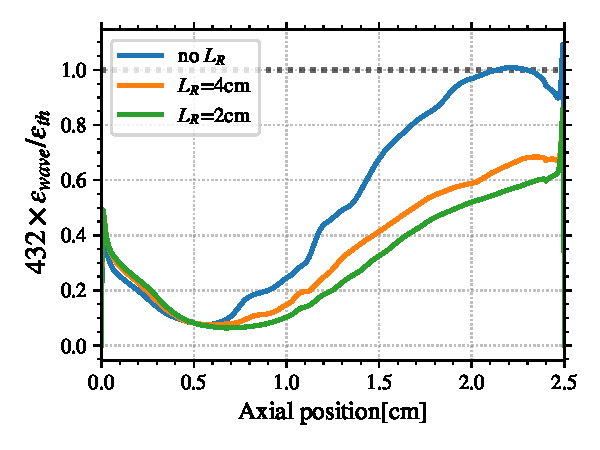
\includegraphics[width=\defaultwidth]{Boeuf_Axial_IonTrapping_criter}
  \caption{Axial evolution of the ion-wave trapping criteria average between $t=6\,\micro\second$ and $t=10\,\micro\second$ for the three cases using the model of Boeuf. }
  \label{fig-ionwavetrapping_axial}
\end{figure}

The reason of this reduction of the wave amplitude due to the radial losses is not determined.
It could be simply due to the modification of the wave growth rate, compared to the wave convection velocity. 
But the numerical noise induced by the radial loss algorithm.
Indeed, the algorithm used here assures a quasi-neutrality at the level of the CPU domain  (approximately \nth{1/400} of the domain size).
As the strictly local quasineutrality is not assured, a numerical noise similar to the one study in \cref{ch-1} in the radial-azimuthal simulation can be present. 

